% Mestre em LaTeX - v0.5
% Copyleft 2008-2013 Bruno C. Vellutini - http://organelas.com/
%
% Permission is hereby granted, free of charge, to any person obtaining a copy
% of this software and associated documentation files (the "Software"), to deal
% in the Software without restriction, including without limitation the rights
% to use, copy, modify, merge, publish, distribute, sublicense, and/or sell
% copies of the Software, and to permit persons to whom the Software is
% furnished to do so, subject to the following conditions:
%
% THE SOFTWARE IS PROVIDED "AS IS", WITHOUT WARRANTY OF ANY KIND, EXPRESS OR
% IMPLIED, INCLUDING BUT NOT LIMITED TO THE WARRANTIES OF MERCHANTABILITY,
% FITNESS FOR A PARTICULAR PURPOSE AND NONINFRINGEMENT. IN NO EVENT SHALL THE
% AUTHORS OR COPYRIGHT HOLDERS BE LIABLE FOR ANY CLAIM, DAMAGES OR OTHER
% LIABILITY, WHETHER IN AN ACTION OF CONTRACT, TORT OR OTHERWISE, ARISING FROM,
% OUT OF OR IN CONNECTION WITH THE SOFTWARE OR THE USE OR OTHER DEALINGS IN
% THE SOFTWARE.
%
% Ou seja, utilize e modifique os arquivos como desejar.
% 
% Para mais informações visite http://nelas.github.com/mestre-em-latex/

% Classe do documento
\documentclass[twoside,a4paper,11pt]{report}


% Pacotes e comandos customizados
%%% Pacotes utilizados %%%

%% Codificação e formatação básica do LaTeX
% Suporte para português (hifenação e caracteres especiais)
\usepackage[english,brazilian]{babel}

% Codificação do arquivo
\usepackage[utf8]{inputenc}

% Mapear caracteres especiais no PDF
\usepackage{cmap} 

% Codificação da fonte
\usepackage[T1]{fontenc}
% Usa a lmodern por padrão (caso cm-super não esteja instalada).
\usepackage{lmodern}

%% Microtipografia
% Utiliza recursos como espaçamento entre letras e entre linhas
\usepackage{microtype}
% Habilita protrusão e expansão, ignorando
% compatibilidade (ver documentação do pacote)
\microtypesetup{activate={true,nocompatibility}}
% factor=1100 aumenta a protrusão (default 1000)
% stretch=10 diminui o valor máximo de expansão (default 20)
% shrink=10 diminui o valor máximo de encolhimento (default 20)
\microtypesetup{factor=1100, stretch=10, shrink=10}
% Tracking, espaçamento entre palavras, kerning
\microtypesetup{tracking=true, spacing=true, kerning=true}
% Remover tracking para Small Caps
\SetTracking{encoding={T1}, shape=sc}{0}
% Remove ligaduras para o 'f'. Se necessário, adicionar letras
% separadas por vírgulas
\DisableLigatures[f]{encoding={T1}}
% Documento em versão "final", suporte para outros idiomas
\microtypesetup{final, babel}

% Essencial para colocar funções e outros símbolos matemáticos
\usepackage{amsmath,amssymb,amsfonts,textcomp}

%% Layout
% Customização do layout da página, margens espelhadas
\usepackage[twoside]{geometry}
% Aumenta as margens internas para espiral
\geometry{bindingoffset=10pt}
% Só pra ajustar o layout
\setlength{\marginparwidth}{90pt}
%\usepackage{layout}

% Para definir espaçamento entre as linhas
\usepackage{setspace} 

% Espaçamento do texto para o frame
\setlength{\fboxsep}{1em}

% Faz com que as margens tenham o mesmo tamanho horizontalmente
%\geometry{hcentering}

%% Elementos Gráficos
% Para incluir figuras (pacote extendido)
\usepackage[]{graphicx} 

%% Suporte a cores
\usepackage{color}
% Os argumentos declaram nomes novos, como Cyan e Crimson
% (ver documentação do pacote).
\usepackage[usenames,dvipsnames,svgnames]{xcolor}

% Criar figura dividida em subfiguras
\usepackage{subfig}
\captionsetup[subfigure]{style=default, margin=0pt, parskip=0pt, hangindent=0pt, indention=0pt, singlelinecheck=true, labelformat=parens, labelsep=space}

% Caso queira guardar as figuras em uma pasta separada
% (descomente e) defina o caminho para o diretório:
%\graphicspath{{./figuras/}}

% Customizar as legendas de figuras e tabelas
\usepackage{caption}

% Criar ambientes com 2 ou mais colunas
\usepackage{multicol}

% Ative o comando abaixo se quiser colocar figuras de fundo (e.g., capa)
%\usepackage{wallpaper}
% Exemplo para inserir a figura na capa está no arquivo pre.tex (linha 7)
% Ajuste da posição da figura no eixo Y
%\addtolength{\wpYoffset}{-140pt}
% Ajuste da posição da figura no eixo X
%\addtolength{\wpXoffset}{36pt}

%% Tabelas
% Elementos extras para formatação de tabelas
\usepackage{array}

% Tabelas com qualidade de publicação
\usepackage{booktabs}

% Para criar tabelas maiores que uma página
\usepackage{longtable}

% adicionar tabelas e figuras como landscape
\usepackage{lscape}

%% Lista de Abreviações
% Cria lista de abreviações
\usepackage[notintoc,portuguese]{nomencl}
\makenomenclature

%% Notas de rodapé
% Lidar com notas de rodapé em diversas situações
\usepackage{footnote}

% Notas criadas nas tabelas ficam no fim das tabelas
\makesavenoteenv{tabular}

% Conta o número de páginas
\usepackage{lastpage}

%% Referências bibliográficas e afins
% Formatar as citações no texto e a lista de referências
\usepackage{natbib}

% Adicionar bibliografia, índice e conteúdo na Tabela de conteúdo
% Não inclui lista de tabelas e figuras no índice
\usepackage[nottoc,notlof,notlot]{tocbibind}

%% Pontuação e unidades
% Posicionar inteligentemente a vírgula como separador decimal
\usepackage{icomma}

% Formatar as unidades com as distâncias corretas
\usepackage[tight]{units}

%% Cabeçalho e rodapé
% Controlar os cabeçalhos e rodapés
\usepackage{fancyhdr}
% Usar os estilos do pacote fancyhdr
\pagestyle{fancy}
\fancypagestyle{plain}{\fancyhf{}}
% Limpar os campos do cabeçalho atual
\fancyhead{}
% Número da página do lado esquerdo [L] nas páginas ímpares [O] e do lado direito [R] nas páginas pares [E]
\fancyhead[LO,RE]{\thepage}
% Nome da seção do lado direito em páginas ímpares
\fancyhead[RO]{\nouppercase{\rightmark}}
% Nome do capítulo do lado esquerdo em páginas pares
\fancyhead[LE]{\nouppercase{\leftmark}}
% Limpar os campos do rodapé
\fancyfoot{}
% Omitir linha de separação entre cabeçalho e conteúdo
\renewcommand{\headrulewidth}{0pt}
% Omitir linha de separação entre rodapé e conteúdo
\renewcommand{\footrulewidth}{0pt}
% Altura do cabeçalho
\headheight 15pt

% Dados do projeto
\newcommand{\nomedoaluno}{Hudson Chaves Costa}
\newcommand{\titulo}{Três Ensaios em Microfinanças e Inclusão Financeira}

%% Links dinâmicos
% Suporte para hipertexto, links para referências e figuras
\usepackage{hyperref}
% Configurações dos links e metatags do PDF a ser gerado
\hypersetup{colorlinks=true, linkcolor=blue, citecolor=blue, filecolor=blue, pagecolor=blue, urlcolor=green,
            pdfauthor={\nomedoaluno},
            pdftitle={\titulo},
            pdfsubject={Assunto do Projeto},
            pdfkeywords={palavra-chave, palavra-chave, palavra-chave},
            pdfproducer={LaTeX},
            pdfcreator={pdfTeX}}

%% Inserir comentários no texto
% Marcar mudanças e fazer comentários
%\usepackage[margins]{trackchanges}
% Iniciais do autor
%\renewcommand{\initialsTwo}{bcv}
% Notas na margem interna
%\reversemarginpar

%% Comandos customizados

% Espécie e abreviação
\newcommand{\subde}{\emph{Clypeaster subdepressus}}
\newcommand{\subsus}{\emph{C.~subdepressus}}

%% Pacotes não implementados
% Para não sobrar espaços em branco estranhos
%\widowpenalty=1000
%\clubpenalty=1000

% Início do texto
\usepackage{Sweave}
\begin{document}
\Sconcordance{concordance:mestrado.tex:mestrado.Rnw:%
1 26 1}
\Sconcordance{concordance:mestrado.tex:./meta.Rnw:ofs 27:%
1 189 1}
\Sconcordance{concordance:mestrado.tex:mestrado.Rnw:ofs 217:%
29 2 1 1 0 1 1}
\Sconcordance{concordance:mestrado.tex:./pre.Rnw:ofs 222:%
1 217 1}
\Sconcordance{concordance:mestrado.tex:./cap1.Rnw:ofs 440:%
1 41 1}
\Sconcordance{concordance:mestrado.tex:./cap2.Rnw:ofs 482:%
1 206 1}
\Sconcordance{concordance:mestrado.tex:./final.Rnw:ofs 689:%
1 6 1}
\Sconcordance{concordance:mestrado.tex:mestrado.Rnw:ofs 696:%
37 7 1}
\Sconcordance{concordance:mestrado.tex:./apendice.Rnw:ofs 704:%
1 4 1}
\Sconcordance{concordance:mestrado.tex:mestrado.Rnw:ofs 709:%
46 2 1}

% Limpa cabeçalhos.
% (solução para lidar com a númeração das páginas pré-textuais).
\pagestyle{empty}

%% Capa
\begin{titlepage}

% Se quiser uma figura de fundo na capa ative o pacote wallpaper
% e descomente a linha abaixo.
% \ThisCenterWallPaper{0.8}{nomedafigura}

\begin{center}
{\LARGE \nomedoaluno}
\par
\vspace{200pt}
{\Huge \titulo}
\par
\vfill
\textbf{{\large Porto Alegre}\\
{\large \the\year}}
\end{center}
\end{titlepage}

% Faz com que a página seguinte sempre seja ímpar (insere pg em branco)
\cleardoublepage

% Numeração em elementos pré-textuais é opcional (ativada por padrão).
% Para desativá-la comente a linha abaixo.
%\pagestyle{fancy}

% Números das páginas em algarismos romanos
\pagenumbering{roman}

%% Página de Rosto

% Numeração não deve aparecer na página de rosto.
\thispagestyle{empty}

\begin{center}
{\LARGE \nomedoaluno}
\par
\vspace{200pt}
{\Huge \titulo}
\end{center}
\par
\vspace{90pt}
\hspace*{175pt}\parbox{7.6cm}{{\large Projeto de Tese apresentado ao Programa de Pós-Graduação em Economia da Universidade Federal do Rio Grande do Sul na Área de Economia Aplicada.}}

\par
\vspace{1em}
\hspace*{175pt}\parbox{7.6cm}{{\large Orientador: Prof. Dr. Sabino Porto da Silva Júnior}}

\par
\vfill
\begin{center}
\textbf{{\large Porto Alegre}\\
{\large \the\year}}
\end{center}

\newpage

% Ficha Catalográfica
%\hspace{8em}\fbox{\begin{minipage}{10cm}
%Aluno, Nome C.

%\hspace{2em}\titulo

%\hspace{2em}\pageref{LastPage} páginas

%\hspace{2em}Dissertação (Mestrado) - Instituto de Biociências da Universidade de São Paulo. Departamento de XXXXXXXX.

%\begin{enumerate}
%\item Palavra-chave
%\item Palavra-chave
%\item Palavra-chave
%\end{enumerate}
%I. Universidade de São Paulo. Instituto de Biociências. Departamento de XXXXXXXX.

%\end{minipage}}
%\par
%\vspace{2em}
%\begin{center}
%{\LARGE\textbf{Comissão Julgadora:}}

%\par
%\vspace{10em}
%\begin{tabular*}{\textwidth}{@{\extracolsep{\fill}}l l}
%\rule{16em}{1px}   & \rule{16em}{1px} \\
%Prof. Dr. 		& Prof. Dr. \\
%Nome			& Nome
%\end{tabular*}

%\par
%\vspace{10em}

%\parbox{16em}{\rule{16em}{1px} \\
%Prof. Dr. \\
%Nome do Orientador}
%\end{center}

%\newpage

% Dedicatória
% Posição do texto na página
%\vspace*{0.75\textheight}
%\begin{flushright}
  %\emph{Dedicatória...}
%\end{flushright}

%\newpage

% Epígrafe
%\vspace*{0.4\textheight}
%\noindent{\LARGE\textbf{Exemplo de epígrafe}}
% Tudo que você escreve no verbatim é renderizado literalmente (comandos não são interpretados e os espaços são respeitados)
%\begin{verbatim}
%O que é bonito?
%É o que persegue o infinito;
%Mas eu não sou
%Eu não sou, não…
%Eu gosto é do inacabado,
%O imperfeito, o estragado, o que dançou
%O que dançou…
%Eu quero mais erosão
%Menos granito.
%Namorar o zero e o não,
%Escrever tudo o que desprezo
%E desprezar tudo o que acredito.
%Eu não quero a gravação, não,
%Eu quero o grito.
%Que a gente vai, a gente vai
%E fica a obra,
%Mas eu persigo o que falta
%Não o que sobra.
%Eu quero tudo que dá e passa.
%Quero tudo que se despe,
%Se despede, e despedaça.
%O que é bonito…
%\end{verbatim}
%\begin{flushright}
%Lenine e Bráulio Tavares
%\end{flushright}

%\newpage

% Agradecimentos

% Espaçamento duplo
%\doublespacing

%\noindent{\LARGE\textbf{Agradecimentos}}

%Agradeço ao meu orientador, ao meu co-orientador, aos meus colaboradores, aos técnicos, à seção administrativa, à fundação que liberou verba para minhas pesquisas, aos meus amigos, à minha família e ao meu grande amor.

%\newpage

%\vspace*{10pt}
% Abstract
%\begin{center}
  %\emph{\begin{large}Resumo\end{large}}\label{resumo}
%\vspace{2pt}
%\end{center}
% Pode parecer estranho, mas colocar uma frase por linha ajuda a organizar e reescrever o texto quando necessário.
% Além disso, ajuda se você estiver comparando versões diferentes do mesmo texto.
% Para separar parágrafos utilize uma linha em branco.
%\noindent
%Esta, quem sabe, é a parte mais importante do seu trabalho.
%É o que a maioria das pessoas vai ler (além do título).
%Seja objetivo sem perder conteúdo.
%Um bom resumo explica porquê este trabalho é interessante, relata como foi feito, o que foi encontrado, contextualiza os resultados e delineia conclusões.
%\par
%\vspace{1em}
%\noindent\textbf{Palavras-chave:} palavra1, palavra2, palavra3
%\newpage

% Criei a página do abstract na mão, por isso tem bem mais comandos do que o resumo acima, apesar de serem idênticas.
%\vspace*{10pt}
% Abstract
%\begin{center}
  %\emph{\begin{large}Abstract\end{large}}\label{abstract}
%\vspace{2pt}
%\end{center}

% Selecionar a linguagem acerta os padrões de hifenação diferentes entre inglês e português.
%\selectlanguage{english}
%\noindent
%This is the most important part of your work.
%This is what most people will read.
%Be concise without omitting content.
%A good abstract explains why this is an interesting study, tells how it was done, what was found, contextualizes the results and set conclusions.
%\par
%\vspace{1em}
%\noindent\textbf{Keywords:} word1, word2, word3

% Voltando ao português...
%\selectlanguage{brazilian}

%\newpage

% Desabilitar protrusão para listas e índice
\microtypesetup{protrusion=false}

% Lista de figuras
\listoffigures

% Lista de tabelas
\listoftables

% Abreviações
% Para imprimir as abreviações siga as instruções em 
% http://code.google.com/p/mestre-em-latex/wiki/ListaDeAbreviaturas
\printnomenclature

% Índice
\tableofcontents

% Re-habilita protrusão novamente
\microtypesetup{protrusion=true}
% Faz com que o ínicio do capítulo sempre seja uma página ímpar
\cleardoublepage

% Inclui o cabeçalho definido no meta.tex
\pagestyle{fancy}

% Números das páginas em arábicos
\pagenumbering{arabic}

\chapter{INTRODUÇÃO}\label{intro}

Há décadas diversas pesquisas teóricas têm focado na fundamentação microeconômica da rigidez de preços, um elemento chave nas explicações dos efeitos reais da política monetária. Por outro lado, a literatura empírica sobre rigidez de preços é pouco encontrada. \citet{bils2004some} fizeram uma importante contribuição ao estudar de forma desagregada dados do \emph{Consumer Price Index} (CPI) dos EUA a partir de 1990 e mostrar que o preço médio mudou uma vez a cada 4.3 meses. Embora outras significantes contribuições seguiram este trabalho, importantes questões empíricas permanecem em grande parte sem resposta.

\citet{cavallo2010scraped} em seu trabalho inovador, fez questionamentos sobre os fundamentos da rigidez de preços. Entre eles, se as decisões de preço são temporalmente dependentes ou relacionada ao estado econômico subjacente, se a rigidez de preços é realmente conduzida por custo de menu e assimetria de informação, o papel da competição e sincronização dos preços e como o ambiente econômico, experiências passadas de inflação e quadros institucionais influenciam na forma como os preços se ajustam.

A principal restrição para pesquisa empírica é que os dados em nível de produto são limitados em termos de frequência, países e contextos em que eles são coletados. Dados do CPI dos EUA e Europa têm se tornado viáveis para pesquisadores em uma base limitada. Embora esses bancos de dados cubram uma vasta gama de produtos, eles são tipicamente viáveis para países desenvolvidos com ambiente macroeconômico estável, onde choques agregados são leves e os mecanismos relevantes em nível micro com objetivos macro são difíceis de identificar. 

Por fim, para conseguir grande quantidade de informações em periodicidade diária, é preciso utilizar a capacidade que a tecnologia proporciona. Além disso, dados tradicionais de pesquisas de instituições públicas e privadas não possuem tais características e assim, são limitantes para pesquisas empíricas sobre o impacto de políticas monetárias e rigidez de preços.

O presente projeto de tese propõe a utilização da tecnologia de web scraping assim como \citet{cavallo2010scraped} para coletar dados de sites de diversos setores da economia brasileira. Assim, pretende-se contribuir para a pesquisa empírica no mercado brasileiro no que tange à avaliação empírica da rigidez de preços e também gerar um índice de inflação que possa ser considerado proxy para os índices divulgados pelo governo. 

\pagestyle{empty}
\cleardoublepage
\pagestyle{fancy}

\chapter{REVISÃO BIBLIOGRÁFICA}\label{cap2}

Como já mencionado anteriormente, pesquisas empíricas que busquem avaliar a rigidez de preços tem pouca audiência em função da dificuldade de acesso a dados de preços de produtos e serviços em uma frequência considerável. O presente projeto de tese tem como objetivo avaliar se dados coletados da nuvem de diversos sites (supermercados, postos de gasolina, farmácias, ...) são capazes de contribuir para o estudo empírico da rigidez de preços. 

O tema ainda é pouco explorado na academia, mas a difusão da internet e a facilidade de acesso via telefones celulares, por exemplo, são fatores que sinalizam para a importância que as informações armazenadas nas páginas de sites têm para estudos econômicos. 

O \emph{Billion Prices Project} (BPP) no \emph{Massachusetts Institute of Technology} (MIT) é uma iniciativa acadêmica que usa preços coletados diariamente de varejistas com lojas online em todo o mundo para conduzir pesquisa econômica. O projeto tem sido uma fonte de dados para diversas pesquisas acadêmicas no que tange à rigidez de preços, impacto de união monetária nos preços relativos internacionais, taxas de câmbios reais, lei do preço único, inflação online versus inflação oficial de países emergentes onde as medidas divulgadas para esta variável são questionadas pelo mercado, comportamento dos preços e oferta de produtos em desastres naturais como os terremotos do Chile em 2010 e Japão em 2011.

\citet{cavallo2010scraped} apresenta de forma inovadora a utilização de dados diários de preços individuais coletados de páginas de supermercados na Argentina, Brasil, Chile e Colômbia entre outubro de 2007 a outubro de 2008 para a avaliar o comportamento microeconômico dos preços e sua implicação para modelos macroeconômicos. O autor apresenta fatos estilizados sobre a rigidez dos preços nestes quatro países e mostram que a distribuição do tamanho da mudança nos preços é bimodal (com algumas alterações próximas a zero por cento). As funções de risco agregado são inclinadas para cima ou em forma côncava, e existe sincronização de mudanças nos preços para marcas concorrentes. Esses fatores desafiam visões comumente vistas na literatura de rigidez de preços que tem sido influenciada por trabalhos teóricos anteriores. 
  
Além disso, \citet{cavallo2010scraped} providencia um índice de inflação alternativo para a Argentina onde estatísticas oficiais tem se tornado irreal para muitas pessoas. Eles mostraram que a inflação anual era consistentemente duas ou três vezes maior do que o índice oficial divulgado. 

 \citet{cavallo2012currency} utilizaram um conjunto de dados de preços online de bens idênticos vendidos em dezenas de países por quatro dos maiores varejistas globais (Apple, IKEA, H\&M, ZARA) para estudar a taxa de câmbio real e seus comportamentos agregados. Em contraste com a literatura, demonstraram que a lei do preço único (LPU) se matem dentro da zona do euro para dez dos milhares de bens vendidos pelos quatro varejistas em três industrias não relacionadas, implicando taxa de juro real igual a um.

Não obstante, \citet{cavallo2012currency} mostraram que desvios da LPU são significativamente maiores para esses mesmos produtos em países com diferentes moedas, mesmo se sua taxa de câmbio real é indexada. Por exemplo, preços na zona do euro diferem tipicamente daqueles na Suécia, que tem uma taxa de câmbio flutuante e também daqueles na Dinamarca, que vincula sua moeda ao euro. Isto esclarece que a moeda comum por si e não simplesmente a falta de volatilidade nominal, é importante na redução da dispersão dos preços entre países. Além disso, a LPU com os EUA se mantem mais para países dolarizados como Equador e El Salvador do que para países como Hong Kong ou Jordânia, que tem suas próprias moedas, mas vinculadas ao dólar americano. 

\citet{cavallo2013prices}	estudaram o comportamento dos preços diários de supermercados e disponibilidade de produtos seguindo dois desastres naturais recentes: terremoto no Chile em 2010 e terremoto no Japão em 2011. Em ambos os casos existiu um efeito imediato e persistente sobre a disponibilidade de produtos. O número de bens disponíveis para venda caiu 32\% no Chile e 17\% no Japão a partir do dia do desastre para seus pontos mais baixos, que ocorreram 61 e 18 dias depois dos terremotos, respectivamente. A disponibilidade de produtos recuperou lentamente e uma significante parte dos bens permaneceram sem estoque depois de seis meses. Ao contrário, os preços ficaram estáveis por meses até mesmo para os bens que estavam experimentando grave carência. Essas tendências estão presentes para todos os níveis de agregação, mas existe heterogeneidade entre categorias. Ainda, \citet{cavallo2013prices} para a frequência e magnitude nas mudanças de preços em ambos os países e encontraram que os resultados no Chile são consistentes com modelos de precificação onde varejistas tem medo da “ira do cliente”. No Japão a evidência sugere um maior papel para a ruptura de distribuição que restringe a capacidade dos varejistas em distribuir após o terremoto. 

Recentemente, \citet{cavallo2014price} refletiram sobre as implicações de um país aderir a uma área de moeda comum nos preços relativos. Os autores consideraram o caso da Letónia, que recentemente deixou sua taxa de câmbio indexada e se juntou à zona do euro em janeiro de 2014. O artigo é o primeiro a usar dados de alta frequência para demonstrar que aderir a uma união monetária tem implicações econômicas para os preços dos países e a taxa de câmbio real. Tal experimento é particularmente útil porque a entrada da Letónia à zona do euro não carregou consigo profundas mudanças nas políticas governamentais. 

Utilizando preços de milhares de bens vendidos pela Zara (coletados via web scraper), a maior varejista de roupas do mundo, os autores observaram que a dispersão dos preços na Letónia desmoronou rapidamente após a adoção do euro. O percentual de bens com preços quase idênticos em Letónia e Alemanha aumentou de 6\% para 89\%. Por outro lado, a tamanho mediano do preço declinou de 7\% para 0\%. Se um número maior de firmas também se comporta desta maneira, esses resultados sugerem que se tornar membro de uma união monetária tem significante implicações para a taxa de câmbio real de países. 


\pagestyle{empty}
\cleardoublepage
\pagestyle{fancy}

\chapter{METODOLOGIA}\label{cap3}

\section*{WEB SCRAPING}

O surgimento da internet, em particular a Web (\emph{Web Wide Word}) trouxe um crescimento exponencial nas disposições de informações. Embora muitas dessas informações sejam úteis, elas raramente estão de uma forma que podemos utilizá-las, pois ainda é comum pessoas gastarem horas na coleta manual de dados de páginas da web.
Especificamente, apesar de disponibilidade, poucos trabalhos acadêmicos em Economia utilizam desta fonte de dados para análise econômica empírica. Tal característica pode ser dada pela dificuldade dos pesquisadores na área em lidar com linguagem de programação que demandam maior conhecimento de computação. Em recente publicação, \citet{varian2014big} salienta que as técnicas utilizadas na Ciência da Computação e outras áreas correlatas para manipular e analisar dados, têm muito a oferecer. \citet{varian2014big} defende que economistas deveriam conhecer melhor esses métodos e usá-los em seus trabalhos. Além disso, \citet{varian2014big} cita a comumente colaboração entre os departamentos de Ciência da Computação e Estatística nas universidades dos EUA. Porém, o autor espera que em um futuro próximo os estudantes de econometria tenham maior colaboração com esses perfis. 

Uma metodologia que facilita o processo de coleta de dados da web é conhecida como \emph{web scraping} que envolve escrever algoritmos que executam automaticamente o que nós fazemos manualmente quando navegamos por uma página de um site de e-commerce, por exemplo. Outro ponto favorável é a pouca necessidade de conhecimentos prévios de programação. 

Segundo \citet{manning2008introduction} \emph{web scraping} é o processo de tirar informações desestruturadas de páginas da web e transformá-las em informações estruturadas que podem ser usadas para análise.  Pelo fato do processo ser tão genérico, é difícil dizer quando o primeiro web scraper foi escrito. Assim, como \citet{cavallo2010scraped}, apresenta-se o \emph{web scraping} como uma alternativa para acessar preços de sites de supermercados, farmácias, postos de gasolina, bancos, imobiliárias, companhia de energia elétrica, lojas de e-commerce, lojas de roupas e calçados, consertos em geral, plano de saúde, escolas particulares, cursos de línguas, entre outros. 

A tecnologia para coletar os preços é simples. A maior parte das páginas são construídas usando uma linguagem de codificação estruturada chamada de \emph{HyperText Markup Language} (HTML). Este código tem “\emph{tags}”, tais como $<center>$ e $<bold>$, que determinam o estilo e localização do texto em uma página. Estas \emph{tags} tendem a permanecer constantes ao longo do tempo, uma vez que proporcionam um “\emph{look and feel}” distinto para cada página. Por contraste, a informação dentro dessas \emph{tags}, tais como preço de produtos, mudam ao longo do tempo. O software de \emph{scraping} pode ser ensinado a utilizar as \emph{tags} em HTML pata localizar informações relevantes sobre um produto e guarda-las em um banco de dados. A repetição desse processo todos os dias produz um banco de dados em formato de painel com um registro por produto por dia. Em adição, o endereço da página (URL) onde cada produto é localizado pode ser usado para classificar produtos em categorias padronizadas. 

Na figura ~\ref{fig:01}, mostramos como o processo de coletar os preços ocorrerá:

\begin{figure}[htbp]
  \centering
  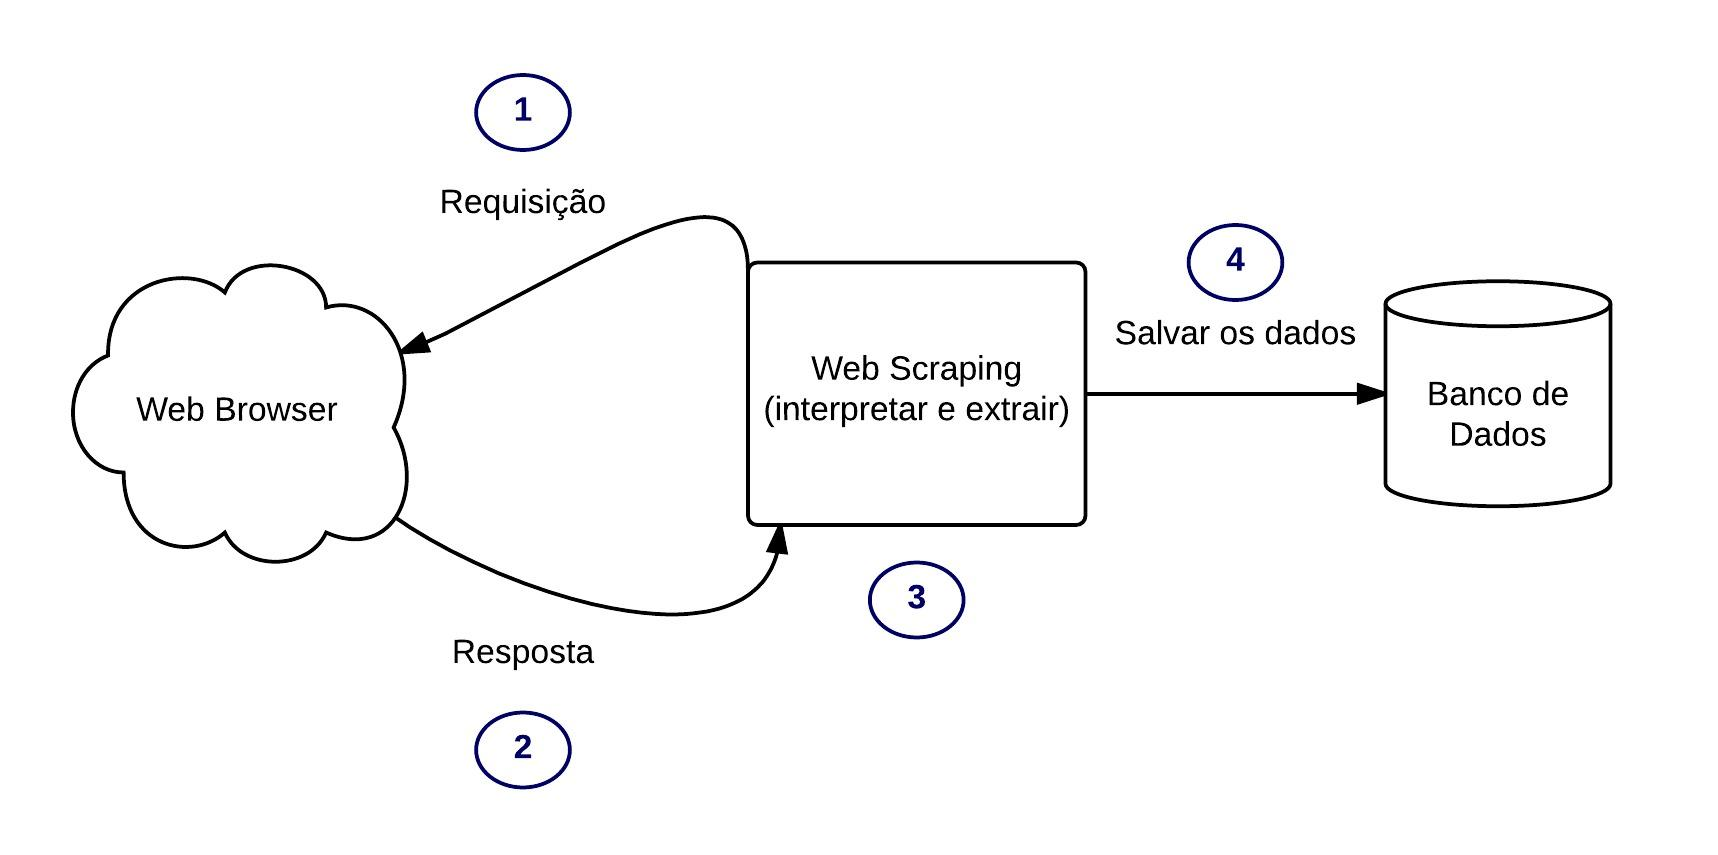
\includegraphics[width=\textwidth]{WebScraping}
  \caption[Figura Simples]{Figura abstrata simples com largura igual à do texto}
  \label{fig:01}
\end{figure}

Segundo \citet{cavallo2010scraped}, preços coletados da internet possuem duas desvantagens: Primeiro, percentual menor de empresas disponibiliza seus produtos e preços na internet em comparação com as lojas físicas. Tal limitação pode ser minimizada ao longo do tempo com uma maior oferta de produtos e serviços na internet. Segundo, os preços coletados da internet não incluem informações sobre as quantidades vendidas o que impede de obter market share e estimativas de elasticidade.

  Não obstante, \citet{cavallo2010scraped} apresenta algumas vantagens dos preços coletados da internet que os fazem uma fonte única de informação para análise de rigidez nos preços. Primeiro, pode-se obter preços diários para os produtos e serviços e por conseguinte, reduzir medidas de erro em relação à frequência de cálculo da inflação, analisar promoções de produtos, controles e sincronização nos preços. Segundo, os dados estão disponíveis para vários países, com maior facilidade de acesso e possibilidade de comparação entre países. Terceiro, existem informações detalhadas sobre cada produto e não há substituições forçada de itens como ocorre em estatísticas oficiais de inflação. Por fim, preços coletados da internet estão viáveis em tempo real, sem qualquer atraso para acessá-los. Isto pode ser usado para providenciar estimativas de rigidez nos preços em tempo real.
  
\section*{ÍNDICE DE PREÇOS ONLINE}
  
  Para calcular o índice de preços online que será comparado com o Índice Nacional de Preços ao Consumidor Amplo (IPCA) Índice Nacional de Preços ao Consumidor (INPC) divulgados pelo Instituto Brasileiro de Geografia e Estatística (IBGE), utilizaremos a abordagem proposta por \citet{cavallo2010scraped}.
  
  Assim, o índice de preços usa a combinação de dados online e as estruturas de ponderação oficiais do IBGE para as categorias da “cesta de mercadorias”\footnote[1]{Segundo o IBGE (2012) os índices constituem uma medida síntese de movimento de preços de um conjunto de bens e serviços, chamado “cesta de mercadorias”, representativo de um determinado grupo populacional, em certo período de tempo} de cada índice de inflação. Dados diários serão utilizados para construir o índice de preços online o que é útil para observar padrões de curto prazo nos dados que ajudam a validar as informações online. 
  
  O índice de preço online será calculado utilizando os preços de todos os produtos disponíveis para compra em cada site. Isto implica que a cesta de bens muda dinamicamente ao longo do tempo podendo um produto aparecer ou desaparecer da cesta a qualquer momento devido à disponibilidade ou indisponibilidade no site. Além disso, o número de preços por produto tende a ser muito maior o que os coletados usualmente pelos órgãos governamentais. 
Para construir o índice, mudanças de preço são calculadas em nível de produto, então as médias dentro das categorias usando média geométrica ponderada e finalmente agregado entre categorias com uma média aritmética ponderada. Em particular, o primeiro passo é obter a média geométrica ponderada das mudanças nos preços na categoria $j$ para cada dia $t$:

\begin{equation}
R_{t,t-1}^{j}=\prod_{i}\left(\frac{p_{t}^{t}}{p_{t-1}^{i}}\right)^{\nicefrac{1}{n_{j,t}}}
\end{equation}

\noindent onde $p_{t}^{i}$ é o preço do bem $i$ no tempo $t$, $n_{j,t}$ é o número de produtos na categoria $j$ que estão presentes na amostra neste dia. 

O segundo passo é computar o índice em nível de categoria em $t$:

\begin{equation}\label{eq2}
I_{t}^{j}=R_{1,0}^{j}\ast{R}_{2,1}^{j}\ast{...}\ast{R}_{t,t-1}^{j}
\end{equation}

Finalmente, o índice de preços no tempo $t$ é a média aritmética ponderada de todos os índices das categorias:

\begin{equation}
IPO_{t}=\sum_{j}{\frac{w_{j}}{w}I_{t}^{j}} 
\end{equation}

\noindent onde $w^{j}$ é o peso oficial utilizado pelo IBGE para tal categoria e $W$ a soma de todos os pesos incluídos na amostra.

A classificação de produtos e pesos de categorias é uma das partes mais complexas deste processo. Nos dados originais, cada produto é atrelado à um endereço de web (URL) que corresponde à página onde o produto é localizado. 

%  O índice de preço online será calculado utilizando os preços de todos os produtos disponíveis para compra em cada site. Isto implica que a cesta de bens muda dinamicamente ao longo do tempo podendo um produto aparecer ou desaparecer da cesta a qualquer momento devido à disponibilidade ou indisponibilidade no site. Além disso, o número de preços por produto tende a ser muito maior o que os coletados usualmente pelos órgãos governamentais. 
% Para construir o índice, mudanças de preço são calculadas em nível de produto, então as médias dentro das categorias usando média geométrica ponderada e finalmente agregado entre categorias com uma média aritmética ponderada. Em particular, o primeiro passo é obter a média geométrica ponderada das mudanças nos preços na categoria $j$ para cada dia $t$



% \SweaveInput{final.Rnw}

% Formato da bibliografia
\bibliographystyle{apalike}

% Arquivo .bib
\bibliography{projeto}

% Apêndice(s)
\appendix

\chapter{Primeiro apêndice}\label{ap2}

Apêndices são opcionais, mas podem ser usados, por exemplo, para incluir tabelas com os dados brutos.

% Fim do texto
\end{document}
